\section{Realna števila, statistika}

\begin{frame}
    \sectionpage
\end{frame}

\begin{frame}
    \tableofcontents[currentsection, hideothersubsections]
\end{frame}

    \subsection{Realna števila}

        \begin{frame}
            \frametitle{Realna števila}
        \end{frame}

    \subsection{Kvadratni in kubični koren}

        \begin{frame}
            \frametitle{Kvadratni in kubični koren}
        \end{frame}

        \begin{frame}
            \begin{exampleblock}{Naloga 563}
                Izračunaj in rezultat delno koreni.
                \begin{description}
                    \item<2->[(b)] $\displaystyle 4\sqrt{8}-\left(2\sqrt{5}+3\sqrt{8}\right)\sqrt{10}$
                    \item<3->[(č)] $\displaystyle\left(5\sqrt{3}+2\sqrt{27}\right)\left(\sqrt{75}-4\sqrt{12}+\sqrt{147}\right)$
                    \item<4->[(g)] $\displaystyle 8\sqrt{3}\left(\sqrt{2}-1\right)-\left(\sqrt{5}+2\sqrt{6}\right)\left(4-2\sqrt{2}\right)$  
                    \item<5->[(j)] $\displaystyle\left(2-4\sqrt{3}\right)\cdot 3\sqrt{2}-\left(2\sqrt{2}-3\sqrt{3}\right)^2$
                    \item<6->[(l)] $\displaystyle\left(3-2\sqrt{2}\right)^3-\left(\sqrt{8}-5\sqrt{2}\right)\left(-3\sqrt{2}\right)$
                    \item<7->[(o)] $\displaystyle\sqrt{300}-\sqrt{5-2\sqrt{6}}\cdot\sqrt{5+2\sqrt{6}}+\sqrt{5^4}$
                    \item<8->[(r)] $\displaystyle\sqrt{5\sqrt{3}-5}\cdot\sqrt{2\sqrt{3}+2}-\left(\sqrt{5}\right)^3$  
                    \item<9->[(u)] $\displaystyle\left(\sqrt{17}-3\right)\sqrt{26+6\sqrt{17}}-\sqrt{2}\left(\sqrt{2}+\sqrt{6}\right)$
                \end{description}
            \end{exampleblock}
        \end{frame}

    \subsection{Intervali}

        \begin{frame}
            \frametitle{Intervali}

            \only<2->{\begin{alertblock}{}
                \textbf{Interval} je množica vseh realnih števil, ki ležijo med dvema danima številoma $a$ in $b$, $a<b$. \\
                Števili $a$ in $b$ imenujemo \textbf{krajišči intervala}.                
            \end{alertblock}
            }

            \only<3->{\begin{block}{Vključenost krajišč}
                \begin{itemize}
                    \item<4-> Simbola $"["$ in $"]"$ označujeta krajišče, ki spada k intervalu.
                    \item<5-> Simbola $"("$ in $")"$ označujeta krajišče, ki ne spada k intervalu.
                \end{itemize}
            \end{block}
            }

            \only<6->{\begin{block}{}
                Pri zapisu intervalov moramo biti pozorni na zapis vrstnega reda števil, ki določata krajišči.
                $$[a,b]\neq[b,a]$$
            \end{block}
            }

            \note{
                Ponazoritev krajišča na številski premici:
                \begin{itemize}
                    \item odebeljena pika / črtica -- krajišče spada k intervalu;
                    \item puščica -- krajišče ne spada k intervalu.
                \end{itemize}
            }

        \end{frame}

        \begin{frame}
            \frametitle{Vrste intervalov}

            \only<2->{\begin{alertblock}{Zaprti interval}
                \only<3->{$$ \mathbf{[a,b]=\left\{x\in\mathbb{R}; a\leq x\leq b\right\} }$$

                \centering
                    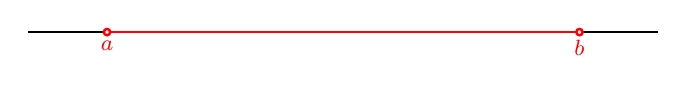
\begin{tikzpicture}
                    % \clip (0,0) rectangle (14.000000,10.000000);
                    {\footnotesize
                    
                    % Drawing line a b
                    \draw [line width=0.016cm] (1.000000,1.500000) -- (1.960000,1.500000);%
                    \draw [line width=0.016cm] (2.040000,1.500000) -- (7.960000,1.500000);%
                    \draw [line width=0.016cm] (8.040000,1.500000) -- (9.000000,1.500000);%
                    
                    % Changing color 255 0 0
                    \definecolor{r255g0b0}{rgb}{1.000000,0.000000,0.000000}%
                    \color{r255g0b0}% 
                    
                    % Drawing segment a b
                    \draw [line width=0.032cm] (2.040000,1.500000) -- (7.960000,1.500000);%
                    
                    % Marking point a by circle
                    \draw [line width=0.032cm] (2.000000,1.500000) circle (0.040000);%
                    \draw (2.000000,1.500000) node [anchor=north] { $a$ };%
                    
                    % Marking point b by circle
                    \draw [line width=0.032cm] (8.000000,1.500000) circle (0.040000);%
                    \draw (8.000000,1.500000) node [anchor=north] { $b$ };%
                    \color{black}
                    }
                    \end{tikzpicture}

                    
                Vsebuje vsa realna števila med $a$ in $b$, vključno s krajiščema $a$ in $b$.
                }
            \end{alertblock}
            }

            \only<4->{\begin{alertblock}{Odprti interval}
                \only<5->{$$ \mathbf{(a,b)=\left\{x\in\mathbb{R}; a<x<b\right\} }$$

                \centering
                    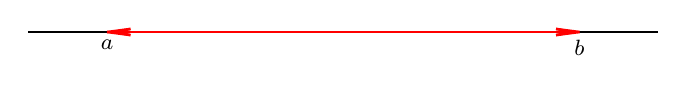
\begin{tikzpicture}
                    % \clip (0,0) rectangle (14.000000,10.000000);
                    {\footnotesize
                    
                    % Drawing line a b
                    \draw [line width=0.016cm] (1.000000,1.500000) -- (9.000000,1.500000);%
                    
                    % Changing color 255 0 0
                    \definecolor{r255g0b0}{rgb}{1.000000,0.000000,0.000000}%
                    \color{r255g0b0}% 
                    
                    % Drawing segment a b
                    \draw [line width=0.032cm] (2.000000,1.500000) -- (8.000000,1.500000);%
                    
                    % Drawing arrow a b 1.00
                    \draw [line width=0.032cm] (7.702567,1.539158) -- (8.000000,1.500000);%
                    \draw [line width=0.032cm] (7.702567,1.539158) -- (7.900856,1.500000);%
                    \draw [line width=0.032cm] (7.702567,1.460842) -- (8.000000,1.500000);%
                    \draw [line width=0.032cm] (7.702567,1.460842) -- (7.900856,1.500000);%
                    
                    % Drawing arrow b a 1.00
                    \draw [line width=0.032cm] (2.297433,1.460842) -- (2.000000,1.500000);%
                    \draw [line width=0.032cm] (2.297433,1.460842) -- (2.099144,1.500000);%
                    \draw [line width=0.032cm] (2.297433,1.539158) -- (2.000000,1.500000);%
                    \draw [line width=0.032cm] (2.297433,1.539158) -- (2.099144,1.500000);%
                    \color{black}
                        
                    % Marking point a
                    \draw (2.000000,1.500000) node [anchor=north] { $a$ };%
                    
                    % Marking point b
                    \draw (8.000000,1.500000) node [anchor=north] { $b$ };%
                    }
                    \end{tikzpicture}
 
                Vsebuje vsa realna števila med $a$ in $b$, vendar ne vsebuje krajišč $a$ in $b$.
                }
            \end{alertblock}
            }

        \end{frame}

        \begin{frame}
            
            \only<2->{\begin{alertblock}{Polodprti/polzaprti interval}
                \begin{itemize}
                    \item<3-> $$ \mathbf{[a,b)=\left\{x\in\mathbb{R}; a\leq x<b\right\} }$$
                    
                    \begin{center}
                        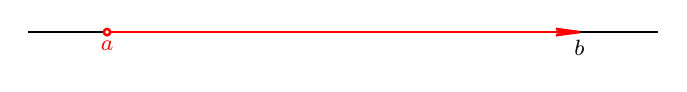
\begin{tikzpicture}
                        % \clip (0,0) rectangle (14.000000,10.000000);
                        {\footnotesize
                        
                        % Drawing line a b
                        \draw [line width=0.016cm] (1.000000,1.500000) -- (1.960000,1.500000);%
                        \draw [line width=0.016cm] (2.040000,1.500000) -- (9.000000,1.500000);%
                        
                        % Changing color 255 0 0
                        \definecolor{r255g0b0}{rgb}{1.000000,0.000000,0.000000}%
                        \color{r255g0b0}% 
                        
                        % Drawing segment a b
                        \draw [line width=0.032cm] (2.040000,1.500000) -- (8.000000,1.500000);%
                        
                        % Marking point a by circle
                        \draw [line width=0.032cm] (2.000000,1.500000) circle (0.040000);%
                        \draw (2.000000,1.500000) node [anchor=north] { $a$ };%
                        
                        % Drawing arrow a b 1.00
                        \draw [line width=0.032cm] (7.702567,1.539158) -- (8.000000,1.500000);%
                        \draw [line width=0.032cm] (7.702567,1.539158) -- (7.900856,1.500000);%
                        \draw [line width=0.032cm] (7.702567,1.460842) -- (8.000000,1.500000);%
                        \draw [line width=0.032cm] (7.702567,1.460842) -- (7.900856,1.500000);%
                        \color{black}
                        
                        % Marking point b
                        \draw (8.000000,1.500000) node [anchor=north] { $b$ };%
                        }
                        \end{tikzpicture}
                    \end{center}

                        
                    Vsebuje vsa realna števila med $a$ in $b$, vključno s krajiščem $a$, vendar ne vsebuje krajišča $b$.
                    

                    \item<4-> $$ \mathbf{(a,b]=\left\{x\in\mathbb{R}; a<x\leq b\right\} }$$
                    
                    \begin{center}
                        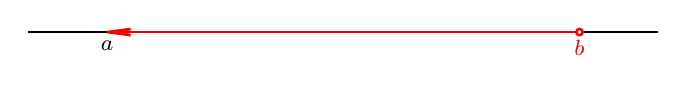
\begin{tikzpicture}
                        % \clip (0,0) rectangle (14.000000,10.000000);
                        {\footnotesize
                        
                        % Drawing line a b
                        \draw [line width=0.016cm] (1.000000,1.500000) -- (7.960000,1.500000);%
                        \draw [line width=0.016cm] (8.040000,1.500000) -- (9.000000,1.500000);%
                        
                        % Changing color 255 0 0
                        \definecolor{r255g0b0}{rgb}{1.000000,0.000000,0.000000}%
                        \color{r255g0b0}% 
                        
                        % Drawing segment a b
                        \draw [line width=0.032cm] (2.000000,1.500000) -- (7.960000,1.500000);%
                        
                        % Marking point b by circle
                        \draw [line width=0.032cm] (8.000000,1.500000) circle (0.040000);%
                        \draw (8.000000,1.500000) node [anchor=north] { $b$ };%
                        
                        % Drawing arrow b a 1.00
                        \draw [line width=0.032cm] (2.297433,1.460842) -- (2.000000,1.500000);%
                        \draw [line width=0.032cm] (2.297433,1.460842) -- (2.099144,1.500000);%
                        \draw [line width=0.032cm] (2.297433,1.539158) -- (2.000000,1.500000);%
                        \draw [line width=0.032cm] (2.297433,1.539158) -- (2.099144,1.500000);%
                        \color{black}

                        % Marking point a
                        \draw (2.000000,1.500000) node [anchor=north] { $a$ };%
                        }
                        \end{tikzpicture}
                    \end{center}

                        
                    Vsebuje vsa realna števila med $a$ in $b$, vključno s krajiščem $b$, vendar ne vsebuje krajišča $a$.

                \end{itemize}


            \end{alertblock}
            }
        \end{frame}

        \begin{frame}
            \only<2->{\begin{alertblock}{Neomejeni/neskončni intervali}
                
                \begin{itemize}
                    \item<3-> $ \mathbf{[a,\infty)=\left\{x\in\mathbb{R}; x\geq a\right\} }$ \\
                    \begin{center}
                        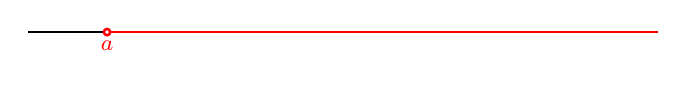
\begin{tikzpicture}
                        % \clip (0,0) rectangle (14.000000,10.000000);
                        {\footnotesize
                        
                        % Drawing line a b
                        \draw [line width=0.016cm] (1.000000,1.500000) -- (1.960000,1.500000);%
                        \draw [line width=0.016cm] (2.040000,1.500000) -- (9.000000,1.500000);%
                        
                        % Changing color 255 0 0
                        \definecolor{r255g0b0}{rgb}{1.000000,0.000000,0.000000}%
                        \color{r255g0b0}% 
                        
                        % Drawing segment a y
                        \draw [line width=0.032cm] (2.040000,1.500000) -- (9.000000,1.500000);%
                        
                        % Marking point a by circle
                        \draw [line width=0.032cm] (2.000000,1.500000) circle (0.040000);%
                        \draw (2.000000,1.500000) node [anchor=north] { $a$ };%
                        \color{black}
                        }
                        \end{tikzpicture}
                    \end{center}
                        
                    \item<4-> $ \mathbf{(a,\infty)=\left\{x\in\mathbb{R}; x>a\right\} }$ \\
                    \begin{center}
                        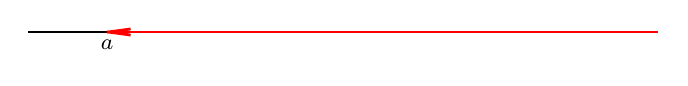
\begin{tikzpicture}
                        % \clip (0,0) rectangle (14.000000,10.000000);
                        {\footnotesize
                        
                        % Drawing line a b
                        \draw [line width=0.016cm] (1.000000,1.500000) -- (9.000000,1.500000);%
                        
                        % Marking point a
                        \draw (2.000000,1.500000) node [anchor=north] { $a$ };%
                        
                        % Changing color 255 0 0
                        \definecolor{r255g0b0}{rgb}{1.000000,0.000000,0.000000}%
                        \color{r255g0b0}% 
                        
                        % Drawing segment a y
                        \draw [line width=0.032cm] (2.000000,1.500000) -- (9.000000,1.500000);%
                        
                        % Drawing arrow b a 1.00
                        \draw [line width=0.032cm] (2.297433,1.460842) -- (2.000000,1.500000);%
                        \draw [line width=0.032cm] (2.297433,1.460842) -- (2.099144,1.500000);%
                        \draw [line width=0.032cm] (2.297433,1.539158) -- (2.000000,1.500000);%
                        \draw [line width=0.032cm] (2.297433,1.539158) -- (2.099144,1.500000);%
                        \color{black}
                        }
                        \end{tikzpicture}
                    \end{center}

                        
                    \item<5-> $\mathbf{(-\infty,b]=\left\{x\in\mathbb{R}; x\leq b\right\} }$ \\
                    \begin{center}
                        
\begin{tikzpicture}
                        % \clip (0,0) rectangle (14.000000,10.000000);
                        {\footnotesize
                        
                        % Drawing line a b
                        \draw [line width=0.016cm] (1.000000,1.500000) -- (7.960000,1.500000);%
                        \draw [line width=0.016cm] (8.040000,1.500000) -- (9.000000,1.500000);%
                        
                        % Changing color 255 0 0
                        \definecolor{r255g0b0}{rgb}{1.000000,0.000000,0.000000}%
                        \color{r255g0b0}% 
                        
                        % Marking point b by circle
                        \draw [line width=0.032cm] (8.000000,1.500000) circle (0.040000);%
                        \draw (8.000000,1.500000) node [anchor=north] { $b$ };%
                        
                        % Drawing segment x b
                        \draw [line width=0.032cm] (1.000000,1.500000) -- (7.960000,1.500000);%
                        \color{black}
                        }
                        \end{tikzpicture}
                    \end{center}

                        
                    \item<6-> $ \mathbf{(-\infty,b)=\left\{x\in\mathbb{R}; x<b\right\} }$ \\
                    \begin{center}
                        
\begin{tikzpicture}
                        % \clip (0,0) rectangle (14.000000,10.000000);
                        {\footnotesize
                        
                        % Drawing line a b
                        \draw [line width=0.016cm] (1.000000,1.500000) -- (9.000000,1.500000);%
                        
                        % Marking point b
                        \draw (8.000000,1.500000) node [anchor=north] { $b$ };%
                        
                        % Changing color 255 0 0
                        \definecolor{r255g0b0}{rgb}{1.000000,0.000000,0.000000}%
                        \color{r255g0b0}% 
                        
                        % Drawing segment x b
                        \draw [line width=0.032cm] (1.000000,1.500000) -- (8.000000,1.500000);%
                        
                        % Drawing arrow a b 1.00
                        \draw [line width=0.032cm] (7.702567,1.539158) -- (8.000000,1.500000);%
                        \draw [line width=0.032cm] (7.702567,1.539158) -- (7.900856,1.500000);%
                        \draw [line width=0.032cm] (7.702567,1.460842) -- (8.000000,1.500000);%
                        \draw [line width=0.032cm] (7.702567,1.460842) -- (7.900856,1.500000);%
                        \color{black}
                        }
                        \end{tikzpicture}
                    \end{center}

                    \item<7-> $ \mathbf{(-\infty,\infty)=\left\{x;x\in\mathbb{R}\right\} =\mathbb{R}}$ \\
                    \begin{center}
                        
\begin{tikzpicture}
                            % \clip (0,0) rectangle (14.000000,10.000000);
                            {\footnotesize
                            
                            % Drawing line a b
                            \draw [line width=0.016cm] (1.000000,1.500000) -- (9.000000,1.500000);%
                            
                            % Changing color 255 0 0
                            \definecolor{r255g0b0}{rgb}{1.000000,0.000000,0.000000}%
                            \color{r255g0b0}% 
                            
                            % Drawing segment x y
                            \draw [line width=0.032cm] (1.000000,1.500000) -- (9.000000,1.500000);%
                            \color{black}
                            }
                        \end{tikzpicture}
                    \end{center}

                \end{itemize}

            \end{alertblock}
            }

            \note{
                Zapis podmnožic $\mathbb{R}$ z intervali:
            \begin{itemize}
                \item $\mathbb{R}^+=(0,\infty)$
                \item $\mathbb{R}_0^+=[0,\infty)$
                \item $\mathbb{R}^-=(-\infty,0)$
            \end{itemize}
            }
        \end{frame}

        \begin{frame}
            \only<2->{\begin{exampleblock}{Naloga 423 (Linea nova)}
                Zapišite množico vseh neengativnih realnih števil, ki so manjša od $6$, ter iskano množico predstavite na številski premici.
            \end{exampleblock}
            \note{Rešitev N423: $\left\{x\in\mathbb{R};0\leq x<6 \right\} [0,6)$ \\}
            }

            \only<3->{\begin{exampleblock}{Naloga 585}
                Dana sta intervala $I=[-2,5)$ in $J=(3,6)$.
                \begin{itemize}
                    % \item Intervala $I$ in $J$ nariši na številski premici.
                    \item<4-> Zapiši $I\cap J$ in $I\cup J$.
                    \item<5-> Izračunaj vsoto največjega celega števila iz $I$ in najmanjšega celega števila iz $J$.
                \end{itemize}
            \end{exampleblock}
            \note{Rešitev N585:\begin{itemize}
                \item $I\cap J=(3,5)$; $I\cup J=[-2,6)$
                \item $4+4=8$
            \end{itemize} }
            }

            \only<6->{\begin{exampleblock}{Naloga 583}
                Zapiši unijo in presek danih intervalov.
                \begin{description}
                    \item[(c)]<7-> $[4,8]$ in $(3,5]$
                    \item[(f)]<8-> $[-2,4]$ in $(2,\infty)$
                    \item[(g)]<9-> $(-\infty,3]$ in $(-1,5]$   
                \end{description}
            \end{exampleblock}
            \note{Rešitev N583: \begin{description}
                \item[(c)] $(3,8]$ in $[4,5]$
                \item[(f)] $[-2,\infty)$ in $(2,4]$
                \item[(g)] $(-\infty,5]$ in $(-1,3]$   
            \end{description}
            }
            }
        \end{frame}

        \begin{frame}
            \frametitle{Linearna neenačba}

            \only<2->{\begin{alertblock}{}
                \textbf{Linearna neenačba} ima v splošnem obliko: $\mathbf{ax+b<cx+d};~ a,b,c,d\in\mathbb{R}$.
            \end{alertblock}
            }

            \only<3->{\begin{block}{Reševanje linearne neenačbe}
                Neenačbo rešimo tako, da ji po korakih prirejamo enostavnejšo ekvivalentno neenačbo, dokler ne pridemo do rešitve.
                Množica rešitev linearne neenačbe je interval, množica intervalov, točka, množica točk ali pa nima rešitve.
            \end{block}
            }

            \only<4->{\begin{block}{Pravila preoblikovanja}
                \begin{itemize}
                    \item<5-> na levi in desni strani neenačbe lahko prištejemo ( ali odštejemo) isto število;
                    \item<6-> levo in desno stran neenačbe lahko pomnožimo z istim (pozitivnim) številom;
                    \item<7-> če levo in desno stran neenačbe pomnožimo z negativnim številom, se znak neenakosti obrne.
                \end{itemize}
            \end{block}
            }

        \end{frame}

        \begin{frame}
            \only<2->{\begin{exampleblock}{Naloga 582}
                Reši neenačbo in rešitev zapiši z intervalom.
                \begin{description}
                    \item[(f)]<3-> $ 2-(2-2x)^2>4x(1-x) $ 
                    \item[(l)]<4-> $ \frac{x+3}{8}\geq \frac{2x-9}{4}  $ 
                    \item[(p)]<5-> $ \frac{x+3}{6}-\frac{2x-1}{12}\leq (3+4)^0+\frac{3x-2}{8} $ 
                \end{description}
            \end{exampleblock}
            \note{Rešitev N582: \begin{description}
                \item[(f)] $x\in(\frac{1}{4},\infty)$
                \item[(l)] $x\in(-\infty,7]$
                \item[(p)] $x\in[-\frac{4}{9},\infty)$  
            \end{description}}
            }

            \only<6->{\begin{exampleblock}{Naloga 584}
                Reši sistem neenačb in rešitev zapiši z intervalom.
                \begin{description}
                    \item[(č)]<7-> $ x+4\leq 8; \quad 5-x<8 $ 
                    \item[(h)]<8-> $ 3-(2+4x)<x^2-(2-x)^2; \quad 2-(2-x)(x+2)\geq x^2 $
                    \item[(e)]<9-> $ 5x-3\geq 4; \quad 11-10x\geq -3 $  
                \end{description}
            \end{exampleblock}
            \note{Rešitev N584: \begin{description}
                \item[(č)] $x\in(-3,4]$
                \item[(h)] ni rešitve
                \item[(e)] $x\in\left\{\frac{7}{5}\right\}$
            \end{description}}
            }

        \end{frame}

        \begin{frame}
            \only<2->{\begin{exampleblock}{Naloga 587}
                Reši neenačbo $4-(2x+3)^3\geq -101-4(x+1)(2x^2+7x)$ v množici:
                \begin{enumerate}[a]
                    \item realnih števil in rešitev ponazori na številski premici,
                    \item naravnih števil in rešitev ponazori na številski premici,
                    \item celih števil in rešitev ponazori na številski premici.
                \end{enumerate}
            \end{exampleblock}
            \note{Rešitev N587:\begin{enumerate}[a]
                \item $x\in(-\infty,3]$
                \item $x\in\left\{1,2,3\right\} $
                \item $x\in\left\{3,2,1,0,-1,-2,\dots\right\} $
            \end{enumerate}}
            }

            \only<3->{\begin{exampleblock}{Naloga 588}
                Dana sta izraza $A=3-(2x-1)^2+4x(x+2)$ in $B=2-\frac{x+1}{3}$. Za katere $x$ je:
                \begin{enumerate}[a]
                    \item<4-> vrednost izraza $A$ negativna,
                    \item<5-> vrednost izraza $B$ vsaj $-88$,
                    \item<6-> vrednost izraza $B$ za $20$ manjša od vrednosti izraza $A$?
                \end{enumerate}
            \end{exampleblock}
            \note{Rešitev N588: \begin{enumerate}[a]
                \item $x\in(-\infty,-\frac{1}{6})$
                \item $x\in(-\infty,269]$
                \item $x\in\left\{\frac{59}{37}\right\} $
            \end{enumerate}}
            }
        \end{frame}


    \subsection{Absolutna vrednost}

        \begin{frame}
            \frametitle{Absolutna vrednost}
        \end{frame}

    \subsection{Sistem linearnih enačb}

        \begin{frame}
            \frametitle{Sistem linearnih enačb}
        \end{frame}

    \subsection{Obravnavanje linearnih enačb, neenačb, sistemov}

        \begin{frame}
            \frametitle{Obravnavanje linearnih enačb, neenačb, sistemov}
        \end{frame}

    \subsection{Absolutna in relativna napaka}

        \begin{frame}
            \frametitle{Absolutna in relativna napaka}
        \end{frame}

    \subsection{Sredine}

        \begin{frame}
            \frametitle{Sredine}
        \end{frame}

    \subsection{Razpršenost podatkov}

        \begin{frame}
            \frametitle{Razpršenost podatkov}
        \end{frame}

    \subsection{Prikazi}
        
        \begin{frame}
            \frametitle{Prikazi}
        \end{frame}